% !TEX root = ../../semexp-thesis.tex

\section{A New Opportunity: Semantic Technologies}
\label{sec:background/semtec}

At the same time, different AI methods for information processing have gained popularity over the last few years that promise better user support in various domains---including programming---by approaching information based on their semantics.
Concretely, we use the term \emph{semantic technologies} to refer two methods, namely \emph{semantic retrieval} using document embeddings and \emph{text generation} using LLMs.

Both technologies approach the semantic information of textual data through the concept of \emph{embeddings}.
An embedding is a numeric representation of a \emph{document} (such as a single word, a text, or also another artifact such as an image) through a high-dimensional vector whose components describe the relatedness of the document to different \emph{features}~\cite{mikolov2013efficient,devlin2019bert}.
Features can represent arbitrary kinds of properties or topics, such as language, sentiment, or length, but in many settings, they are used to encode continuous combinations of various concepts through dimensional reduction.
In this setting, the distance of two embeddings in the vector space indicates the similarity of their associated documents with regard to the employed concepts.
This lays the foundation for performing different arithmetic operations to compare, organize, or sort documents in a given context.

\subsection{The Transformer Architecture}

\begin{figure}[Z]
	\centering
	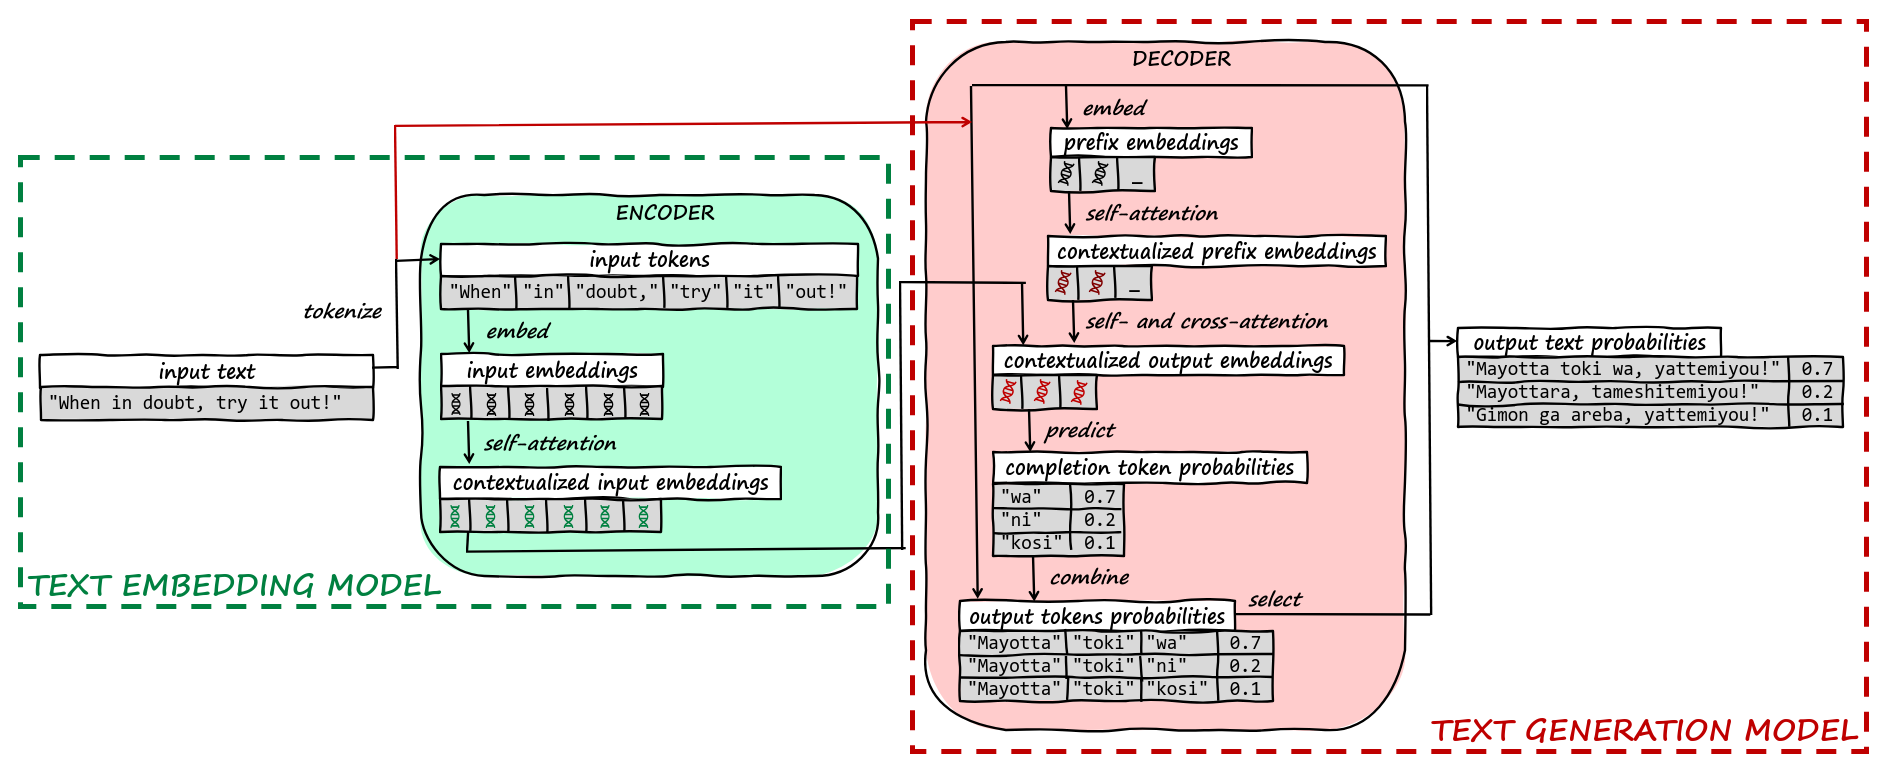
\includegraphics[width=\linewidth]{04_semtec/transformer.png}
	% todo: kreuzende linien überbrücken
	\caption[A high-level overview of the \emph{transformer architecture} for large language models that embed and generate text.]{
		A high-level overview of the transformer architecture, which is used by many language models for translating text from one language (here: English) to another (here: Japanese).
		The encoder computes embeddings for each input token and contextualizes them with each other.
		The decoder sequentially generates the output text based on the input embeddings and the previous output prefix by contextualizing them together and predicting the next token.
		\emph{Text embedding models} only employ the encoder component of a transformer, while many \emph{text generation models} only use the decoder and treat the input text as an output prefix instead.
	}
	\label{fig:background/semtec/transformer}
\end{figure}

The language models that power these semantic technologies---\emph{embedding models} that compute embedding representations of documents and \emph{generative LLMs} that can produce plausible texts (usually referred to as shortly LLMs)---are commonly based on the \emph{transformer architecture}~\cite{vaswani2017attention}%
\footnote{
	We acknowledge the existence of alternative architectures such as long-short term memory (LSTMs), latent semantic analysis (LSA), convolutional neural networks (CNNs), and hybrid approaches but restrict our focus in this short introduction to the transformer architecture, which is used predominantly in modern large general-purpose embedding and text generation models~\cite{oralkbekova2023contemporary}.
}.
Here, we provide a high-level overview of transformer models, focusing on their conceptual operating principles and deliberately omitting mathematical and technical details.

From a macroscopic viewpoint, a transformer model employs several neural networks to translate a text from an input language into a text in an output language~(\cref{fig:background/semtec/transformer}).
Possible languages include natural languages, programming languages, other formal languages, or (sequential representations of) multimedia data such as images.
The model is usually trained by supervised learning using a set of input-output pairs.
Internally, a transformer consists of two components: the \emph{encoder} and the \emph{decoder}:

\begin{description}[noextralabelsep]
	\item[The encoder] converts the input text into a sequence of \emph{contextualized token embeddings}.
	For that, it first splits up the text into a sequence of tokens from a finite alphabet (such as words or parts of words) and embeds these tokens using a pre-learned lookup table.
	It then contextually enriches these embeddings through multiple layers that comprise of a self-attention mechanism and a feed-forward neural network.
	Through self-attention, the different input tokens are put in relation to each other based on multiple aspects such as syntactical, lexical, or positional relationships.
	As a result, the contextualized token embeddings describe the semantics of each token in the context of the input text.

	\begin{example}
		In the text ``Squeak image'', an encoder would embed the token ``Squeak'' closer to other tokens describing programming systems such as ``Smalltalk'' or ``Jupyter''.
		%However, in the sentence ``Squeak and rattle'', the same token would be embedded closer to automative-related tokens such as ``buzz'' or ``NVH''.
		However, in the sentence ``Squeak mouse'', the same token would be embedded closer to toy-related tokens such as ``noise'' or ``rubber''.
	\end{example}

	\item[The decoder] is invoked multiple times with a sequence of contextualized input token embeddings to \emph{infer} or generate a likely output text or a probability distribution of output texts.
	At each invocation, the transformer predicts the next output token given the contextualized input embeddings and all previously generated output tokens.
	It contextually enriches the previous output tokens and combines them with the input embeddings through a self- and cross-attentive stack similar as in the encoder.
	From the contextually enriched output token embeddings, it selects the embedding next to the previous generated token and converts it into a probability distribution of tokens.
	This process is repeated until the output sequence ends with a special end token.
	Through a \emph{beam search}, the transformer can explore multiple paths of the probability tree instead of greedily only considering the most likely token at each step.

	Text inference in the decoder can be configured through several hyperparameters that modify the probability distributions of output tokens:
	for example, a \emph{temperature} factor and a \emph{nucleus sampling rate} can alter or truncate the variance of outputs, often associated with the creativity of the model~\cite{holtzman2020curious}; \emph{frequency penalties} can control the repetitiveness of outputs; or \emph{token biases} can prioritize particular tokens~\footnote{
		OpenAI: ``Text Generation Models''. \emph{OpenAI API Reference.} URL:
		%\url{https://web.archive.org/web/20240530210910/https://platform.openai.com/docs/guides/text-generation/text-generation-models}
		\url{http://archive.today/2024.05.30-211619/https://platform.openai.com/docs/guides/text-generation/text-generation-models}%
		.
	}.
\end{description}

In the following, we describe how transformers are used by embedding models for semantic retrieval and by generative LLMs for text completions.

\subsection{Semantic Retrieval with Embedding Models}
\label{sec:background/semtec/retrieval}

To compute a \emph{document embedding} (also referred to as \emph{sentence embedding} or \emph{text embedding}) of a text, models such as \name{BERT} (bidirectional encoder representations from transformers), \name{XLNet}, and \name{T5} use only the encoder component of transformers that was trained using self-supervised learning and aggregate the resulting embedding sequence into a single embedding vector~\cite{devlin2019bert,raffel2023exploring}.
\emph{Semantic retrieval systems} (also referred to as \emph{vector databases} or \emph{vector stores}) compute and index document embeddings for objects such as web pages, files, or source code~\cite{lewis2020retrieval}.
This allows them to efficiently perform a \emph{similarity search} in order to recommend semantically related objects to a given object.

Semantic retrieval systems can also offer a more general form of \emph{semantic search} by taking a free-form query from a user, embedding it, and comparing it to the existing document embeddings.
Based on the training of the embedding model, this can even yield useful results when query and documents are in different formats; to improve search quality, queries and documents can be transformed into a consistent representation through preprocessing prior to computing embeddings, e.g., by generating possible questions for documents or hypothetical relevant documents (\emph{hypothetical document embeddings}, \name{HyDE})~\cite{mao2021generation,gao2022precise} for questions using static heuristics or another language model.

Other popular applications of document embeddings include clustering (grouping and anomaly detection) and classification (e.g., based on languages or sentiments).

\subsection{Text Generation with LLMs}
\label{sec:background/semtec/generation}

Generative LLMs such as \name{GPT} (generative pre-trained transformer), \name{LLaMA}, and \name{PaLM} use only the decoder component of transformers:
instead of encoding and transforming an input text, they treat it as a part of the output text and generate a likely completion of it~\cite{radford2018improving,openai2024gpt4}.
They are usually trained using a combination of self-supervised learning with large text corpora and reinforcement learning from human feedback (RLHF) to fine-tune completions~\cite{ouyang2022training}.

One of the earliest practical applications of LLMs that had a wider impact on the programming community was integrated \emph{semantic code completion} tools such as GitHub Copilot, Tabnine, CodeWhisperer, and others~\cite{chen2021evaluating,barka2023grounded} that suggest additions to the code a programmer has typed in an editor.

Beyond simple text completion, LLMs can also be trained to adhere to certain text formats and patterns and follow \emph{instructions} in the prompt, allowing the construction of specialized \emph{agents} with different characteristics:

\begin{description}[noextralabelsep]
	\item[Conversational agents] engage in conversations with human \emph{users} by generating messages (that complete a conversation history) on behalf of a virtual \emph{assistant}~\cite{bai2022training}.
	Optionally, \emph{system} messages can be used to provide further instructions to agents.
	For example, OpenAI's ChatGPT, Google Gemini, or GitHub Copilot Chat allow users to write, edit, review, or summarize text or source code or discuss a wide range of topics through a chat interface~\cite{openai2024gpt4}.

	\item[Autonomous agents] are instructed to generate \emph{inner monologues} that mimic structured thinking, resulting in basic capabilities for self-organized problem solving~\cite{yang2023autogpt}.

	Additionally, they can be enabled via pre-training or instructions to access external systems through \emph{function calls}: an LLM emits a special output sequence that requests the invocation of a system function with a set of arguments, a handler executes this invocation and passes back the result with the text to the LLM, and the LLM continues the generation based on the result~\cite{hao2023toolkengpt,mialon2023augmented,yang2023autogpt}.
	For instance, when presented with a mathematical word problem, GPT-4 can break down the task, plan a solution approach, and source out primitive arithmetic tasks to an external calculator function~\cite{openai2024gpt4}.

	Building on the concept of autonomous agents, \emph{multi-agent frameworks} such as \name{MetaGPT} and \name{ChatDev} orchestrate multiple agents that cooperate intending to solve complex problems such as software development~\cite{hong2023metagpt,qian2023communicative}.
\end{description}

Being statistical models without an actual understanding of matters in human terms, LLMs suffer from several weaknesses such as limited logical reasoning, not adhering to instructions, and \emph{hallucinations} where false information is generated~\cite{openai2024gpt4}.
To mitigate these problems in parts, several techniques have been established:

\begin{description}
	\item[Fine-tuning:] Adjust the output style and behavior of models by training a base model on a curated set of positive examples of texts or conversations~\cite{kojima2022large,wei2022finetuned}.

	\item[Prompt engineering:] Adjust the output style and behavior by strategically developing prompts and instructions that are most likely to influence models in an intended way~\cite{white2023prompt}.
	For example, \emph{chain-of-thought} prompting instructs models to explicate their thoughts as inner monologue (``think out aloud'') or expressing upfront plans in a certain structure and has been shown to improve their problem-solving abilities~\cite{wei2023chainofthought}.

	Other than fine-tuning, prompt engineering can be applied to any model without retraining, but the prompt must be presented to the LLM for each generation, affecting its performance~\cite{zhao2023survey}, and often several iterations are required to develop effective prompts~\cite{white2023prompt}.

	\item[Retrieval-augmented generation (RAG):] To mitigate the limited abilities of LLMs to recall rarely seen information or provide them with new information, gather excerpts from external sources through traditional algorithms (such as database lookups and full-text searches) and include them in the prompt~\cite{lewis2020retrieval}.
	This often includes semantic retrieval methods~(see \cref{sec:background/semtec/retrieval}).

	For example, the Microsoft Copilot integration in Bing performs one or a few web searches based on the query of the user, feeds the result into the GPT-4 model, and instructs it to answer the query based on the provided information\footnote{
		Microsoft. 2023-11-21. \emph{How Copilot Works.}
		URL:
		%\url{https://www.microsoft.com/en-us/bing/do-more-with-ai/how-bing-chat-works} (accessed 2024-05-29)
		\url{http://archive.today/2024.05.30-235455/https://www.microsoft.com/en-us/bing/do-more-with-ai/how-bing-chat-works}%
		.
	}.
	Alternatively, agents can also proactively call functions to retrieve required information.
	Thus, RAG reduces the challenge of information recall to filtering, contextualizing, and summarizing presented information or answering questions about it.
\end{description}

\ParSep

Due to their foundations of machine learning methods, semantic technologies make it possible to process and synthetize information based on their context and semantics.
We believe that this creates an opportunity to tackle the limitations of traditional exploratory programming systems which are restricted to technical interfaces at lower abstraction levels.
By integrating semantic technologies into exploratory programming systems, we envision to provide wider-ranging, conceptual, and contextual support for programmers within their exploratory workflow.
